\chapter{System Model and Problem Formulation}\label{cha: System Model and Problem Formulation}

Let us consider a residential home that is connected to the electricity market via the power grid, but is also equipped with renewable energy generators, such as solar panels and wind turbines, and with a battery of size $C$ (kWh) to regulate the energy usage over time. The electricity is purchased from both a day-ahead and a real-time market where the prices may vary over $H$ time slots of the day. The day-ahead and real-time electricity prices are given by $p_d^{\text{DA}}(h)$ and $p_d^{\text{RT}}(h)$ (USD/kWh), respectively, where $d$ is the index of the day and $h\in\{1,2,\ldots, H\}$ represents the time slot within the day. The user employs an energy management system, as illustrated in Figure~\ref{fig: system model}, that determines the amount of day-ahead energy purchase (i.e., the amount of energy to be purchased for the next day) based on the electricity prices, renewable energy arrivals, residential loads and battery levels during the current day. The cost of energy usage consists of the cost of energy purchase from the market as well as the cost of battery usage. First, we formulate the cost of energy purchase  from grid and our system model in secton~\ref{sec: Cost of Energy Purchase}. Second, in Section~\ref{sec: Cost of Battery Usage}, we introduce number of cycle of batteries and define the current depth-of-discharge for each time slot, then, formulate the cost of batteries.

\begin{figure}[ht]
  \centering
  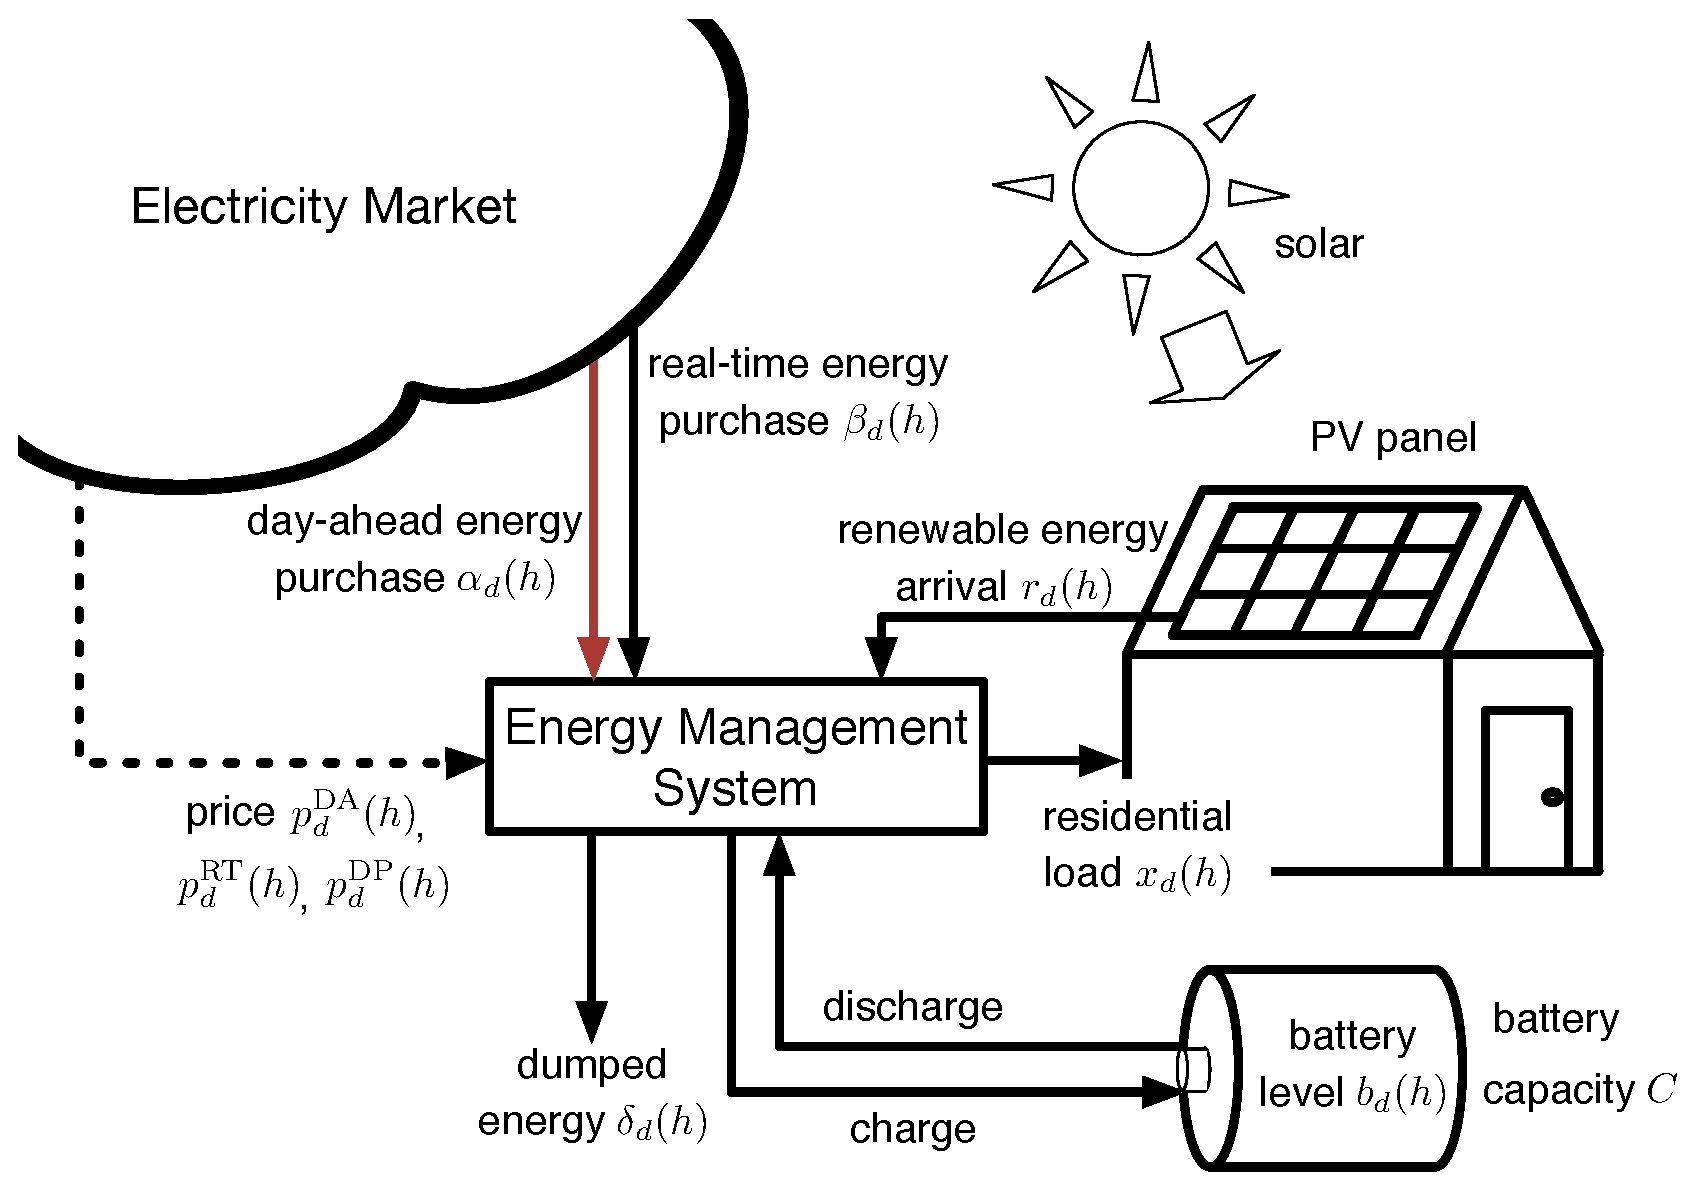
\includegraphics[width=0.8\textwidth]{fig/model.eps}
  \caption{System Model.}
  \label{fig: system model}
\vspace{-.3cm}
\end{figure}

\section{Cost of Energy Purchase}\label{sec: Cost of Energy Purchase}

The cost of energy purchase from grid can be formulate by the energy flow of EMS. Let $r_d(h)$, $x_d(h)$, and $b_d(h)$ be the amount of renewable energy arrival, residential load, and battery level, respectively, at the end of time slot $h$ on day $d$, where $h = 1, 2, \ldots, H$ and $d = 1, 2, \ldots$. The amount of day-ahead purchase, denoted by $\alpha_d(h)$, for $h=1,\ldots, H$, was determined at the end of day $d-1$ based on knowledge of $r_{d-1}(h)$, $x_{d-1}(h)$, and $b_{d-1}(h)$, for all $h$. Due to the uncertainty of the next-day electricity pricing, renewable energy arrival, and residential loads, the day-ahead purchase may be in excess by amount
\begin{equation}\label{eq: excess energy}
    e_d(h) = b_d(h-1) + r_d(h) + \alpha_d(h) - x_d(h)
\end{equation}
where $b_d(0)\triangleq b_{d-1}(H)$. The intuition of \eqref{eq: excess energy} is that the possible energy we can utilize, that is, $b_d(h-1) + r_d(h) + \alpha_d(h)$, minus the residential demand $x_d(h)$. Notice that this excess energy can be either positive or negative depending on whether or not energy is over-purchased or under-purchased in the day ahead market. When the excess energy is positive, it is stored in the battery, resulting in battery level of
\begin{equation}
    b_d(h) = \max\left\{0,\min\left\{e_d(h),C\right\}\right\}
\end{equation}
at the end of time slot $h$. The amount of energy that cannot be stored due to limited battery capacity, i.e.,
\begin{equation}
\delta_d(h) =
\max\left\{0,e_d(h)-C\right\},
\end{equation}
is dumped at the price of $p_d^{\text{DP}}(h)$ (USD/kWh).
When the excess energy is negative, the amount of energy
\begin{equation}
    \beta_d(h) = \max\left\{0,-e_d(h)\right\}
\end{equation}
should be purchased from the real-time market to support the current residential demand. The total cost of purchasing electricity from the market is thus given by
\begin{equation}\label{eq: cost of purchasing electricity from the market}
\kappa^\text{grid}_d(h) = p^\tDA_d(h)\alpha_d(h)+p^\tRT_d(h)\beta_d(h)+p^\text{DP}_d(h)\delta_d(h).
    % \kappa^\text{grid}_d(h) = 0.8 p^\tDA_d(h)\alpha_d(h)+p^\tRT_d(h)\beta_d(h)+p^\text{DP}_d(h)\delta_d(h).
\end{equation}

\section{Cost of Battery Usage}\label{sec: Cost of Battery Usage}

In addition to the cost of energy purchase from the market, the use of battery to regulate energy purchase and usage over time also results in a cost due to battery degradation. In particular, with each charge and discharge cycle, the battery will degrade progressively and the speed of degradation depends on the DoD \cite{linden:1865}, which is defined as the ratio between the total discharge in a cycle and the total battery capacity. In fact, the number of cycles that a battery can be used in a lifetime decreases rapidly as the DoD increases and is given by \cite{dallinger:2013}
\begin{equation}
  N_\text{cycle} = c_1 \cdot \text{DoD}^{-c_2}
\end{equation}
for some constants $c_1$ and $c_2$ that varies for different type of batteries. For a typical Li-ion battery in 2012, the constants are given by $c_1 = 1331$ and $c_2 = 1.825$ \cite{dallinger:2013}. Based on this relation, the residential user may not want to use energy from the battery if the cost of further increasing the DoD is higher than the current electricity price from the market.

To consider the tradeoff between DoD and the battery lifetime, we propose to model the cost of battery usage as the marginal cost of increasing the DoD by the amount of usage. More specifically, let $p_{\text{batt}}$ be the battery price per kWh capacity. Then, for a battery with capacity $C$ and a given DoD in each cycle, the average cost per cycle is given by ${p^\text{batt}\cdot C}/{( c_1 \cdot \text{DoD}^{-c_2})}$. Moreover, by defining the current DoD in time slot $h$ as
\begin{equation}
    \text{cDoD}_d(h)=\frac{1}{C}\sum_{t=h'+1}^h \left(b_{d}(t-1)- b_d(t)\right)
\end{equation}
where $h'=\max\{1\leq t\leq h:b_{d}(t-1)-b_{d}(t)<0\}$\footnote{For notational simplicity, we assume that the discharge does not extend to the previous day since batteries are usually charged at midnight. However, this can be easily extended to the general case with proper choice of notations.}, the marginal cost of battery usage in time slot $h$ can be modeled as
\begin{equation}\label{eq: cost of battery usage}
    \kappa^\text{batt}_d(h) = \max\left\{0, \frac{p^\text{batt}\cdot C}{c_1\cdot\text{cDoD}_d(h)^{-c_2}}-\frac{p^\text{batt}\cdot C}{c_1\cdot\text{cDoD}_d(h-1)^{-c_2}}\right\}
\end{equation}
This novel consideration of the battery cost realistically captures the tradeoff between the DoD and the battery lifetime. The intuition \eqref{eq: cost of battery usage} is that we consider the cost of battery usage in each time slot by compare there average cost per cycle. Moreover, the cost of battery in \eqref{eq: cost of battery usage} grow exponentially when current DoD grow linearly.

Hence, the total cost at time $h$ on day $d$ is given by
\begin{equation}\label{eq: total cost}
    \kappa_d(h) = \kappa^\text{grid}_d(h) + \kappa^\text{batt}_d(h).
\end{equation}
This cost depends on the day-ahead energy purchase $\bfalpha_d\triangleq [\alpha_d(1),\ldots, \alpha_d(H)]^T$ as well as the system states, such as electricity prices, renewable energy arrival, residential load profile, and battery level. Different from most works in the literature that rely on (precise or statistical) knowledge of the above-mentioned system states, we utilize a reinforcement learning based policy iteration method to determine the day-ahead energy management policy using only historical data.
